\documentclass[12pt]{article}
\usepackage{float}
\usepackage{graphicx}
\usepackage{fontspec}
\usepackage{titlesec}
\usepackage{setspace}
\usepackage[style=numeric,backend=biber,sorting=none]{biblatex}
\usepackage[a4paper, total={6in, 8in}, margin=0.5in]{geometry}
\addbibresource{ref.bib}

%%%%%%%% FORMAT
\singlespacing
\setmainfont{Arial}

\titleformat*{\section}{\normalsize\bfseries}
\titleformat*{\subsection}{\normalsize\bfseries}

\pagenumbering{gobble} % Suppress page number

% \titlespacing\section{0pt}{12pt plus 4pt minus 2pt}{0pt plus 2pt minus 2pt}
% \titlespacing\subsection{0pt}{12pt plus 4pt minus 2pt}{0pt plus 2pt minus 2pt}
% \titlespacing\subsubsection{0pt}{12pt plus 4pt minus 2pt}{0pt plus 2pt minus 2pt}


\begin{document}
  
%%%%%%%%% TITLE  
\title{\large Application of micromanipulation techniques in assisted fertilization  \vspace{-2em}}
% \author{\large Yujia Shi\vspace{-1em}}
\date{\vspace{-2.5em}}
\maketitle

%%%%%%%%% BODY TEXT
\section{INTROUDCTION}
micromanipulation is described as a set of tools and techniques that performed on small group of cells or single cells to advacned our understanding in reproductive biology and the development of clinical
methodology.Over the past decade,micromanipulation has played a key role in many scientific discipline, especially in the field of 
assisted fertilization. There is a considerable number of patients unalbe to pregnancy through the conventional in vitro fertilization (IVF) procedure due to failure of fertilization.Various micromanipulation techniques have been developed to assist fertilization, they offer an great effort to address the dilemma of male infertility,they hold great promise for effective diagnosis as well as circumvention of inherited genetic conditions.\medskip


Nowadays, micromanipulation is a field which filled with extensive base of methodology and expertiment, which has been greatly used in variety of reproductive development animal and biology husbandry settings.In the late 1970s, the scientists around the world start to consider the application of micromanipulative techniques in human clincal reproduction. After Steptoe and Edwards have made sucess in  
the  generation an offspring by the conception of in vitro fertillisation, marking a tunning point for assisted reproduction  and  in vitro fertilization in human,since from this event ,various groups all over the world begin to invest more time and efforts in the idea of in vitro fertilization by introducing more complex  techniques of oocyt and embryo manipulation, which bring the hope for patients with severely impaired sperm characteristics, making the sperm more closer or into the ovum.However,to date, there  a relatively large group of patients with poors permatozoal function still can not achieve pregnancy.The remaining failure can be ascribed to the sperm cells are not able to penetrate the zona pellucida and integrate with oolemma. Several procedures have been introduced to  increase the interaction between sperm-egg interaction in the past time such as 
\begin{itemize}
    \item [1)] 
    Either raising the sperm content within the inseminating suspension or decresing the total mass of the insemination medium via the use of microdrops.
    \item [2)] 
    Improving the method of selecting candidate sperm for the purpose of gaining more spermatozoa with normal motibility
    \item [3)]
    facilitating the contact between spermatozoa and moility enhancer as well as isolating the oocyte from the surrounding cumulus cells
\end{itemize}
The above of procedures will be beneficial to treat moderate oligoasthenospermia, but have failed to promote the fertilization in those patients with severely compromised semen parameters.\medskip

Zona pellucida is the main obstacle and natural barrier for normal spermatozoa penetrate into mammalian eggs,this is particularly visible when spermatozoa deficient in density, motility and morphology, the penetration capability to penetrate the zona pellucida will be significantly reduced.
Several techniques have been developed to bypass this thick oocyte's coat.Remove entirely of the zona pellucida exposing spermatozoa to oocyte,however,which may result in low rate of fertilization as well as impair the develpment and survival of the preimplantation embryo.The emergence of micromanipulative techniques designed to enable zona pellucida reaching the oocyte without removal of the entire zona pellucida, which offer some advacne.\medskip


The method Zona drilling was completed through acidic Tyrode’s (AT) medium to create a hole in the zona pellucida, enabling access to oocyte plasma membrane.A similar method to zona drilling is partial zona dissection (PZD) which bring the sperms closer to the female gamete by using mechanical forces to partial open up the human zona pellucida, thereby increasing the interacton between sperm and the oolemma of the oocyte.The partial zone dissection is effective for those oligozoospermic patients,but not meant for asthenozoospermia patients with severse semen problems or immunological infertility.\medskip

A more direct way to assist the fertilization process is the method called  subzonal insemination (SUZI),which involves in the process of placeing fewer spermatozoas straightly  into the perivitelline space,to avoid the incidence of polyspermy.The appearance of subzonal inseminating is somewhat successful, as which have been applied successfully to treat even male with severely impaired sperm characteristics such as impaired progressive motility.Thus,it is superior to partial zona dissection.\medskip

The dominant progression in the field of assisted
fertilization was Intracytoplasmic sperm injection (ICSI).There is doubt that intracytoplasmic sperm injection is currently most outstanding  accomplishment in the field of assisted which is a well established method widely used worldwide to treat infertility.Intracytoplasmic sperm injection was dervied from the onventional in vitro fertilization (IVF),but there is slightly difference between ICSI and IVF. Intracytoplasmic sperm injection designed to inject a single spermatozoon into an oocyte cytoplasm by using a glass micropipette;while for 

The micromanipulation techniques that were developed to assist fertilization
include partial zona dissection (PZD), 

\begin{figure}[H]
    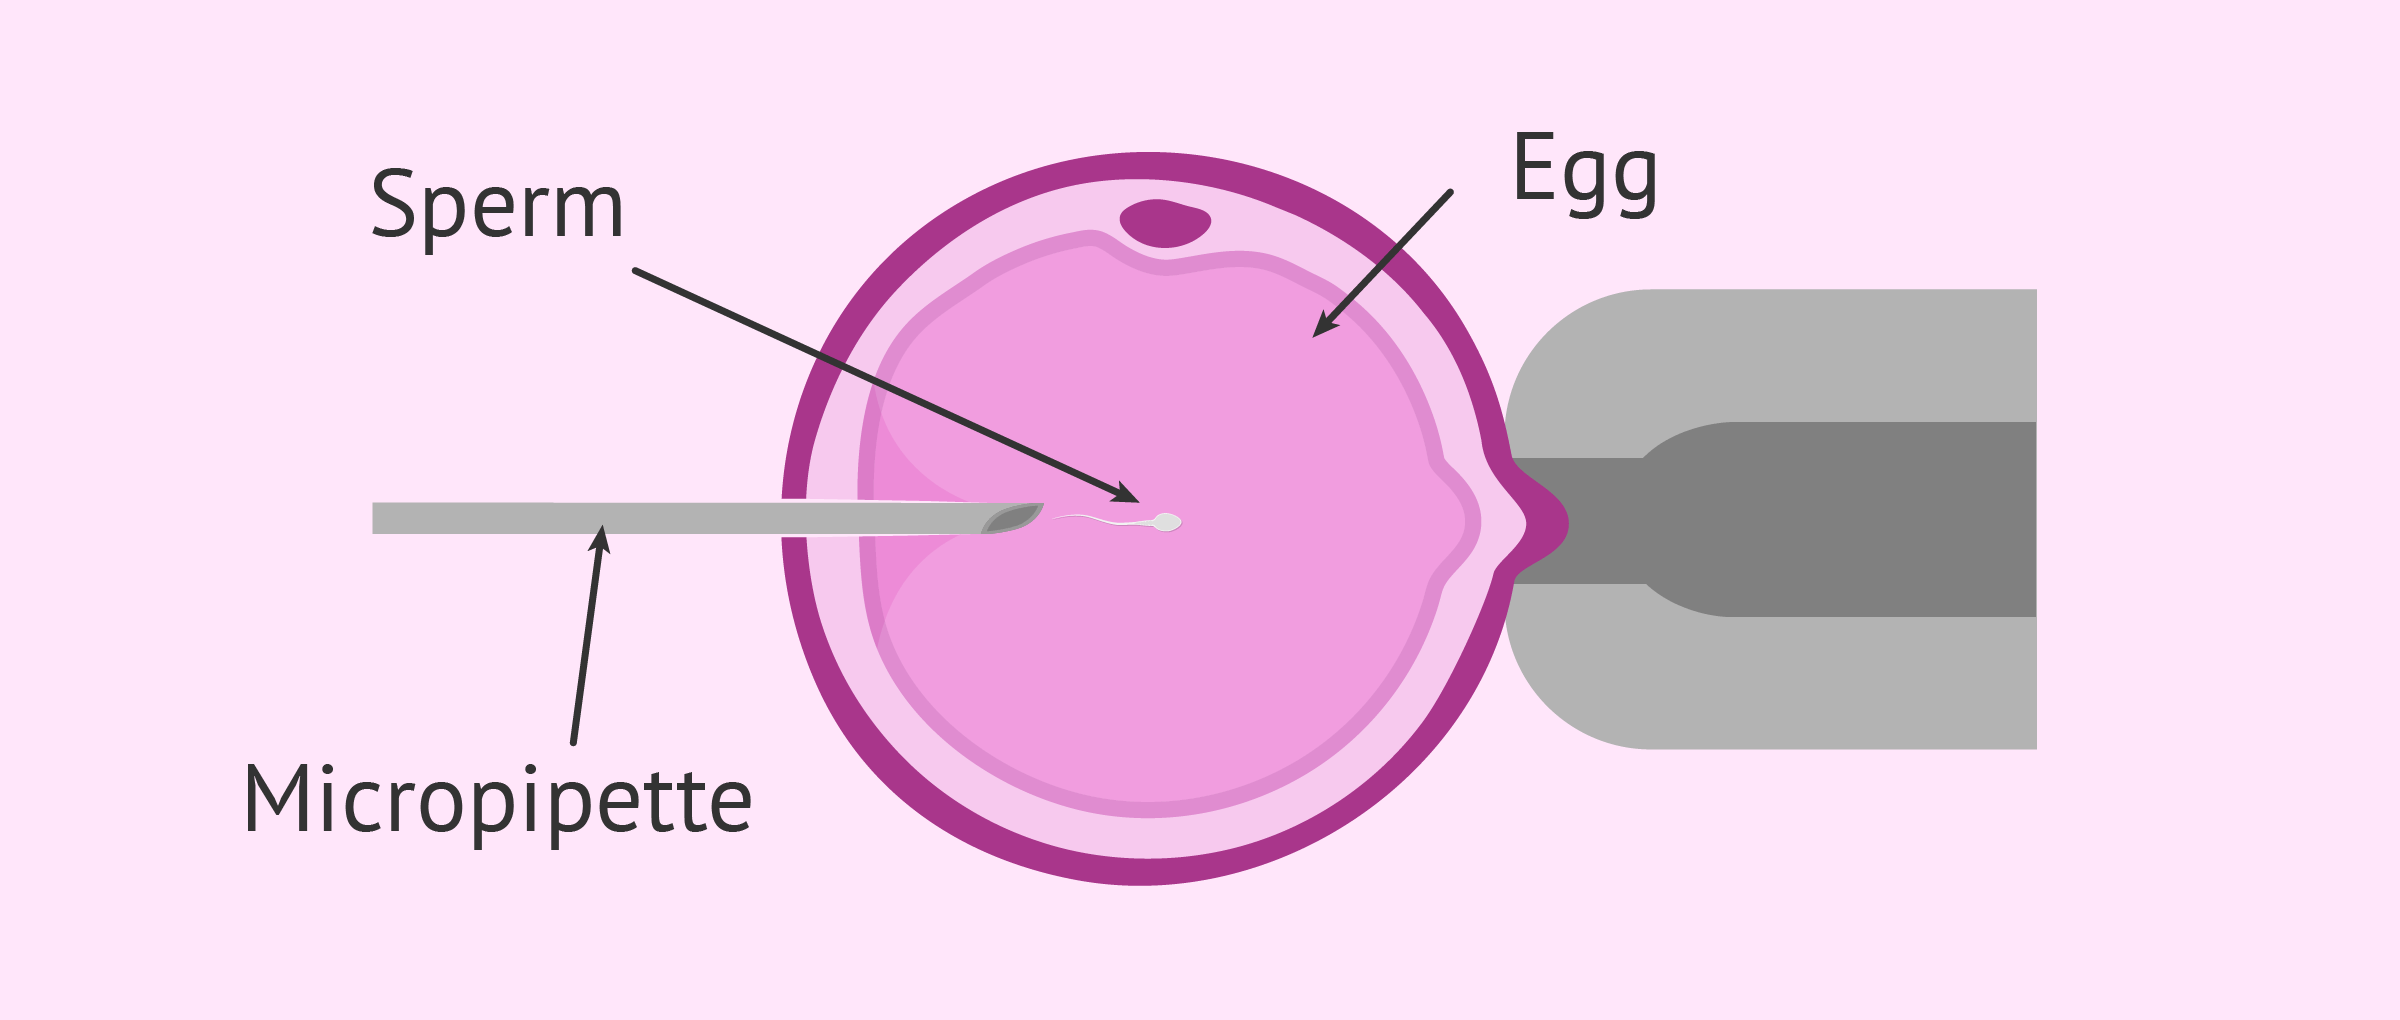
\includegraphics[width=0.8 \linewidth,height=0.45\columnwidth]{/Users/yu-pinglin/Desktop/Essay/6003_kennth.png}
    \centering
    \caption{The 4 pillars for building a sustainable portfolio of
    core facilities.}
\end{figure}









\emergencystretch=1em
\printbibliography[title=Reference]

\end{document}




